\chapter{代数簇上的函数}

本章中，我们将在一个固定的域 \(k\) 上进行讨论.从(4.8, II)节开始，我们将假设 \(k\) 是代数闭域.为方便理解，读者不妨始终假设 \(k = \mathbb{C}\)，这在大部分情况下不会影响结论的本质，甚至可能有助于直观把握.为简化符号，我们有时会省略对基域 \(k\) 的提及.

\section{多项式函数}

设 \(V \subset  {\mathbb{A}}_{k}^{n}\) 是一个代数集，其理想为 \(I(V)\).商环 \(k[V] = k[X_1, \ldots, X_n]/I(V)\) 很自然地成为 \(V\) 上的函数环.

具体而言，我们定义 \(V\) 上的\textbf{多项式函数}（polynomial function）为形如 \(f : V \rightarrow  k\) 的映射，其形式为 \(P \mapsto  F(P)\)，其中 \(F \in  k[X_1, \ldots, X_n]\).这意味着 \(f\) 是由某个多项式 \(F : {\mathbb{A}}^{n} \rightarrow  k\) 在 \(V\) 上的限制.

根据理想 \(I(V)\) 的定义，两个多项式 \(F, G \in  k[X_1, \ldots, X_n]\) 在 \(V\) 上定义了相同的函数，当且仅当
\[
F(P) - G(P) = 0 \text{ 对所有 } P \in  V,
\]
即当且仅当 \(F - G \in  I(V)\).因此，我们定义\textbf{坐标环}（coordinate ring）\(k[V]\) 为：
\[
k[V] = \{ f : V \rightarrow  k \mid  f \text{ 是多项式函数} \} \cong  k[X_1, \ldots, X_n]/I(V).
\]
该环是包含所有坐标函数 \(x_i\) 以及常数域 \(k\) 的最小函数环，因此“坐标环”这一传统术语在此处是相当直观的.

\section{\(k[V]\) 与 \(V\) 的代数子集}

一个代数集 \(X \subset  {\mathbb{A}}^{n}\) 包含于 \(V\) 中，当且仅当 \(I(X) \supset  I(V)\).另一方面，\(k[X_1, \ldots, X_n]\) 中包含 \(I(V)\) 的理想与商环 \(k[X_1, \ldots, X_n]/I(V)\) 的理想之间存在着自然的一一对应关系.（具体来说，理想 \(J\) 满足 \(I(V) \subset  J \subset  k[X_1, \ldots, X_n]\) 对应于商环中的理想 \(J/I(V)\)；反之，\(k[X_1, \ldots, X_n]/I(V)\) 的理想 \({J}_{0}\) 对应于它在 \(k[X_1, \ldots, X_n]\) 中的原像.）

因此，在 \(k[V]\) 的理想与 \(V\) 的子集之间，我们有与第3章类似的 \(I\) 和 \(V\) 对应关系：
\[
V: \{ \text{理想 } I \subset  k[V] \} \to \{ \text{子集 } X \subset  V \}
\]
定义为
\[
I \mapsto  V(I) = \{ P \in  V \mid  f(P) = 0 \text{ 对所有 } f \in  I \},
\]
以及
\[
I: \{ \text{子集 } X \subset  V \} \to \{ \text{理想 } J \subset  k[V] \}
\]
定义为
\[
X \mapsto I(X) = \{ f \in  k[V] \mid  f(P) = 0 \text{ 对所有 } P \in  X \}.
\]
这些对应关系具有类似的性质.特别地，\(V\) 具有Zariski拓扑，其闭集是 \(V\) 的代数子集（这自然是 \({\mathbb{A}}^{n}\) 的Zariski拓扑诱导的子空间拓扑）.

\begin{proposition}
设 \(V \subset  {\mathbb{A}}^{n}\) 是一个代数子集.以下条件等价：
\begin{enumerate}
    \item \(V\) 是不可约的；
    \item \(V\) 的任意两个非空开子集 \({U}_{1}, {U}_{2}\) 的交集非空；
    \item \(V\) 的任意非空开子集 \(U\) 都是稠密的.
\end{enumerate}
\end{proposition}
\begin{proof}
这些都是显然的.\(V\) 不可约意味着 \(V\) 不能表示为两个真闭子集的并.条件(ii)是用补集语言对该定义的等价表述，因为
\[
{U}_{1} \cap  {U}_{2} = \varnothing  \Leftrightarrow  V = (V \setminus {U}_{1}) \cup (V \setminus {U}_{2}).
\]
一个拓扑空间的子集是稠密的，当且仅当它与每个非空开集都有交集，因此(iii)只是(ii)的另一种表述.
\end{proof}

\section{多项式映射}

设 \(V \subset  {\mathbb{A}}^{n}\) 和 \(W \subset  {\mathbb{A}}^{m}\) 为代数集；我们分别用 \({X}_{1},\ldots ,{X}_{n}\) 和 \({Y}_{1},\ldots ,{Y}_{m}\) 表示 \({\mathbb{A}}^{n}\) 和 \({\mathbb{A}}^{m}\) 上的坐标.

\begin{definition}[多项式映射]
一个映射 \(f : V \rightarrow  W\) 称为\textbf{多项式映射}（polynomial map），如果存在 \(m\) 个多项式 \({F}_{1},\ldots ,{F}_{m} \in k[X_1, \ldots, X_n]\)，使得对所有 \(P \in  V\)，
\[
f(P) = (F_1(P), \ldots, F_m(P)) \in {\mathbb{A}}_{k}^{m}.
\]
\end{definition}
这是前述多项式函数概念的直接推广.

\begin{proposition}
映射 \(f : V \rightarrow  W\) 是多项式映射，当且仅当对所有 \(j\)，其第 \(j\) 个坐标函数 \({f}_{j} = {Y}_{j} \circ  f\) 是 \(V\) 上的多项式函数，即 \({f}_{j} \in k[V]\).
\end{proposition}

\begin{center}
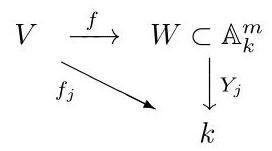
\includegraphics[max width=0.2\textwidth]{images/bo_d3lj80c601uc738kffi0_71_637_1756_272_151_0.jpg}
\end{center}
\hspace*{3em} 

\begin{proof}
这很明显：若 \(f\) 由 \({F}_{1},\ldots ,{F}_{m}\) 给出，则复合映射即为 \(P \mapsto  {F}_{j}(P)\)，它是一个多项式函数.反之，若对每个 \(j\) 都有 \({f}_{j} \in  k[V]\)，则我们可以选取任意 \({F}_{j} \in  k[X_1, \ldots, X_n]\) 使得 \({f}_{j} = {F}_{j} \pmod{I(V)}\)，从而得到 \(f\) 作为由 \((F_1, \ldots, F_m)\) 给出的多项式映射的描述.根据此命题，映射 \(f\) 可写作 \(f = (f_1, \ldots, f_m)\).
\end{proof}

多项式映射的复合以一种自然的方式定义：设 \(V \subset  {\mathbb{A}}^{n}, W \subset  {\mathbb{A}}^{m}\) 和 \(U \subset  {\mathbb{A}}^{\ell}\) 为代数集，且 \(f : V \rightarrow  W, g : W \rightarrow  U\) 为多项式映射，则复合映射 \(g \circ  f : V \rightarrow  U\) 仍然是多项式映射.若 \(f\) 由 \({F}_{1},\ldots ,{F}_{m} \in  k[X_1, \ldots, X_n]\) 给出，且 \(g\) 由 \({G}_{1},\ldots ,{G}_{\ell } \in k[Y_1, \ldots, Y_m]\) 给出，则 \(g \circ  f\) 由以下多项式给出：
\[
{G}_{1}(F_1, \ldots, F_m), \ldots, {G}_{\ell}(F_1, \ldots, F_m) \in  k[X_1, \ldots, X_n].
\]

\begin{definition}[同构]
代数集之间的多项式映射 \(f : V \rightarrow  W\) 称为\textbf{同构}（isomorphism），如果存在一个多项式映射 \(g : W \rightarrow  V\) 使得 \(f \circ  g = \mathrm{id}_W\) 且 \(g \circ  f = \mathrm{id}_V\).
\end{definition}

我们已经见过几个多项式映射的例子：
\begin{itemize}
    \item (2.1)中由 \(t \mapsto  (t^2, t^3)\) 或 \((t^2 - 1, t^3 - t)\) 给出的参数化 \({\mathbb{R}}^{1} \rightarrow  C \subset {\mathbb{R}}^{2}\).
    \item (3.11, b)中由 \(t \mapsto  (t^3, t^4, t^5)\) 定义的映射 \(k \rightarrow  C \subset  {\mathbb{A}}_{k}^{3}\).
    \item 在讨论诺特正规化时，我们有一个代数集 \(V \subset  {\mathbb{A}}_{k}^{n}\)，并考虑了由“相当一般”的线性形式 \({Y}_{1},\ldots ,{Y}_{m}\) 定义的射影 \(p : V \rightarrow  {\mathbb{A}}_{k}^{m}\).由于 \({Y}_{i}\) 是 \({\mathbb{A}}_{k}^{n}\) 上坐标 \({X}_{j}\) 的线性组合，这个射影是一个多项式映射.
\end{itemize}

另一方面，(1.1)中圆的参数化是由有理函数给出的（分母中有一项 \({\lambda }^{2} + 1\)），因此不是多项式映射.同样，从奇异三次曲线 \(C \subset  {\mathbb{R}}^{2}\) 到 \({\mathbb{R}}^{1}\) 的逆映射 \((X,Y) \mapsto  t = Y/X\) 也不是多项式映射.

\section{多项式映射与 \(k[V]\)}

\begin{theorem}
设 \(V \subset  {\mathbb{A}}_{k}^{n}\) 和 \(W \subset  {\mathbb{A}}_{k}^{m}\) 为代数集.
\begin{enumerate}
    \item[\upshape (1)] 一个多项式映射 \(f : V \rightarrow  W\) 诱导一个 \(k\)-代数同态 \({f}^{ * } : k[W] \rightarrow  k[V]\)，该同态由函数复合定义：若 \(g \in  k[W]\) 是一个多项式函数，则 \({f}^{ * }(g) = g \circ  f\) 也是一个多项式函数.映射 \(g \mapsto  g \circ  f\) 定义了一个从 \(k[W]\) 到 \(k[V]\) 的 \(k\)-代数同态.（注意映射方向是反的.）

    \item[\upshape (2)] 反之，任何一个 \(k\)-代数同态 \(\Phi  : k[W] \rightarrow  k[V]\) 都可由一个唯一确定的多项式映射 \(f : V \rightarrow  W\) 诱导，使得 \(\Phi  = {f}^{ * }\).
\end{enumerate}
因此，上述两点表明，通过 \(f \mapsto  {f}^{ * }\) 建立的映射
\[
\left\{ \begin{array}{c} \text{多项式映射} \\ f : V \rightarrow  W \end{array} \right\} \longleftrightarrow \left\{ \begin{array}{c} k\text{-代数同态} \\ \Phi  : k[W] \rightarrow  k[V] \end{array} \right\}
\]
是一个双射.
\begin{enumerate}
    \item[\upshape (3)] 若 \(f : V \rightarrow  W\) 和 \(g : W \rightarrow  U\) 是多项式映射，则复合映射的同态满足 \({\left( g \circ  f\right) }^{ * } = {f}^{ * } \circ  {g}^{ * } : k[U] \rightarrow  k[V]\).
\end{enumerate}
\end{theorem}

\begin{proof}
(1) 根据(4.3)的讨论，\({f}^{ * }(g)\) 是一个从 \(V\) 到 \(k\) 的多项式函数，因此 \({f}^{ * }(g) \in  k[V]\).显然，对所有常数 \(a \in  k\)，\({f}^{ * }(a) = a\).\({f}^{ * }\) 是一个环同态，这是因为 \(k[W]\) 和 \(k[V]\) 都是函数环，其环结构是逐点定义的.例如，对 \({g}_{1},{g}_{2} \in  k[W]\)，和 \({g}_{1} + {g}_{2}\) 定义为对所有 \(P \in  W\)，\((g_1 + g_2)(P) = g_1(P) + g_2(P)\).因此，\({f}^{ * }(g_1 + g_2)(Q) = (g_1 + g_2)(f(Q)) = g_1(f(Q)) + g_2(f(Q)) = {f}^{ * }g_1(Q) + {f}^{ * }g_2(Q)\).

(3) 这仅仅是函数复合满足结合律的体现.

(2) 这部分的表述需要一些技巧，但内容依然是直接的.对 \(i = 1,\ldots ,m\)，令 \({y}_{i} \in  k[W]\) 为 \(W\) 上的第 \(i\) 个坐标函数，因此
\[
k[W] = k[y_1, \ldots, y_m] = k[Y_1, \ldots, Y_m]/I(W).
\]
给定一个 \(k\)-代数同态 \(\Phi  : k[W] \rightarrow  k[V]\)，我们可以定义 \({f}_{i} = \Phi(y_i) \in  k[V]\).

现在考虑由 \(f(P) = (f_1(P), \ldots, f_m(P))\) 定义的映射 \(f : V \rightarrow  {\mathbb{A}}_{k}^{m}\).这是一个多项式映射，因为每个 \({f}_{i}\) 都是 \(k[V]\) 中的元素.我们断言 \(f\) 将 \(V\) 映入 \(W\)，即 \(f(V) \subset  W\).
确实，假设 \(G \in  I(W) \subset  k[Y_1, \ldots, Y_m]\)；那么在环 \(k[W]\) 中，我们有
\[
G(y_1, \ldots, y_m) = 0.
\]
将同态 \(\Phi\) 应用于此等式，得到 \( \Phi(G(y_1, \ldots, y_m)) = 0 \in  k[V]\).由于 \(\Phi\) 是一个 \(k\)-代数同态，
\[
0 = \Phi(G(y_1, \ldots, y_m)) = G(\Phi(y_1), \ldots, \Phi(y_m)) = G(f_1, \ldots, f_m).
\]
这里的 \({f}_{i}\) 是定义在 \(V\) 上的函数，而 \(G(f_1, \ldots, f_m) \in  k[V]\) 是函数 \(P \mapsto  G(f_1(P), \ldots, f_m(P))\).这表明，对任意 \(P \in  V\) 和任意 \(G \in  I(W)\)，点 \(f(P)\) 的坐标 \((f_1(P), \ldots, f_m(P))\) 满足 \(G(f_1(P), \ldots, f_m(P)) = 0\).由于 \(W\) 是由 \(I(W)\) 中多项式的零点定义的，这意味着 \(f(P) \in  W\).

因此，\(f\) 是一个多项式映射 \(f : V \rightarrow  W\).要验证两个 \(k\)-代数同态 \({f}^{ * }\) 和 \(\Phi\) 是否一致，只需检查它们在生成元上的取值.根据 \(f\) 的构造，\({f}^{ * }(y_i) = y_i \circ f = f_i = \Phi(y_i)\)，所以它们是一致的.类似的论证也表明，映射 \(f\) 由条件 \({f}^{ * }(y_i) = \Phi(y_i)\) 唯一确定.
\end{proof}

\begin{corollary}
一个多项式映射 \(f : V \rightarrow  W\) 是同构，当且仅当它诱导的同态 \({f}^{ * } : k[W] \rightarrow  k[V]\) 是一个同构.
\end{corollary}

\paragraph{例子} 在无限域 \(k\) 上，多项式映射
\[
\varphi  : {\mathbb{A}}_{k}^{1} \rightarrow  C : (Y^2 = X^3) \subset  {\mathbb{A}}_{k}^{2} \quad \text{由 } T \mapsto  (T^2, T^3) \text{ 给出}
\]
不是一个同构.因为在这种情况下，同态
\[
{\varphi }^{ * } : k[C] = k[X,Y]/(Y^2 - X^3) \rightarrow  k[T]
\]
由 \(X \mapsto  T^2, Y \mapsto  T^3\) 给出.\({\varphi }^{ * }\) 的像是 \(k[T^2, T^3]\)，这是一个严格小于 \(k[T]\) 的子代数（例如，\(T\) 就不在其像中）.

注意，\(\varphi\) 是一个双射，因此存在一个完美的逆映射 \(\psi  : C \rightarrow  {\mathbb{A}}_{k}^{1}\)，当 \((X,Y) = (0,0)\) 时取值为0，否则为 \(Y/X\).那么为什么 \(\varphi\) 不是同构呢？关键在于 \(C\) 上的多项式函数比 \({\mathbb{A}}^{1}\) 上的要少.直观上讲，\(\varphi\) “压缩”了原点处的切向量.

\section{仿射簇}

设 \(k\) 为一个域.我们希望将\textbf{仿射簇}（affine variety）定义为一个不可约代数子集 \(V \subset  {\mathbb{A}}_{k}^{n}\)，且该定义在同构意义下是明确的.

定理4.4告诉我们，坐标环 \(k[V]\) 是簇 \(V\) 的一个同构不变量.这使我们能够给出一个不那么依赖于嵌入空间 \({\mathbb{A}}_{k}^{n}\) 的簇的定义.这样做的动机比较微妙，如果暂时忽略它，也不会有太大损失.后续对仿射簇的引用将始终采用 \(V \subset {\mathbb{A}}^n\) 的形式.

\begin{definition}
域 \(k\) 上的一个\textbf{仿射簇}是一个集合 \(V\) 以及其上的一个 \(k\)-值函数环 \(k[V]\)，满足：
\begin{enumerate}
    \item \(k[V]\) 是一个有限生成的 \(k\)-代数；
    \item 对于 \(k[V]\) 的某组生成元 \({x}_{1},\ldots ,{x}_{n}\)，映射
    \[
    V \rightarrow  {\mathbb{A}}_{k}^{n} \quad \text{由 } P \mapsto  (x_1(P), \ldots, x_n(P)) \text{ 定义}
    \]
    将 \(V\) 嵌入为一个不可约代数集.
\end{enumerate}
\end{definition}

\section{函数域}

设 \(V\) 为一个仿射簇.其坐标环 \(k[V]\) 是一个整环，其元素是定义在 \(V\) 上的函数.

\begin{definition}
\(V\) 的\textbf{函数域}（function field）\(k(V)\) 是其坐标环 \(k[V]\) 的分式域，即 \(k(V) = \operatorname{Quot}(k[V])\).\(k(V)\) 中的元素 \(f\) 称为 \(V\) 上的\textbf{有理函数}（rational function）.注意，\(f \in  k(V)\) 被定义为一个分式 \(f = g/h\)，其中 \(g,h \in  k[V]\) 且 \(h \neq  0\).
\end{definition}

一个有理函数 \(f\) 先验地并不是在 \(V\) 上处处定义的函数，因为分母 \(h\) 可能有零点.然而，只要 \(h(P) \neq  0\)，\(f\) 在点 \(P \in  V\) 处就是良定义的，因此它至少是一个“部分定义的函数”.

\begin{definition}
设 \(f \in  k(V)\) 和 \(P \in  V\).如果存在一个表达式 \(f = g/h\)，其中 \(g,h \in  k[V]\) 且 \(h(P) \neq  0\)，则称 \(f\) 在 \(P\) 处是\textbf{正则的}（regular），或称 \(P\) 属于 \(f\) 的\textbf{定义域}（domain of definition）.
\end{definition}

需要注意的一个重要事实是，\(k[V]\) 通常不是唯一分解整环（UFD），因此一个有理函数 \(f \in  k(V)\) 可能有本质上不同的分式表示 \(f = g/h\).记
\[
\operatorname{dom}(f) = \{ P \in  V \mid  f \text{ 在 } P \text{ 处正则} \}
\]
为 \(f\) 的定义域.在点 \(P\) 处正则的所有有理函数的集合构成一个子环：
\[
{\mathcal{O}}_{V,P} = \{ f \in  k(V) \mid  f \text{ 在 } P \text{ 处正则} \} = k[V][\{ h^{-1} \mid  h(P) \neq  0 \}],
\]
它被称为 \(V\) 在 \(P\) 处的\textbf{局部环}（local ring）.

\begin{theorem}
(I) \(\operatorname{dom}(f)\) 在Zariski拓扑下是一个非空开集，因而是稠密的.

假设域 \(k\) 是代数闭的，则
(II)
\[
\operatorname{dom}(f) = V \Leftrightarrow  f \in  k[V]
\]
（即，处处正则的有理函数就是多项式函数）.此外，对任意 \(h \in  k[V]\)，设
\[
{V}_{h} = V \setminus  V(h) = \{ P \in  V \mid  h(P) \neq  0 \};
\]
则
(III)
\[
\operatorname{dom}(f) \supset  {V}_{h} \Leftrightarrow  f \in  k[V][h^{-1}].
\]
\end{theorem}

\begin{proof}
定义 \(f \in  k(V)\) 的分母理想为
\[
{D}_{f} = \{ h \in  k[V] \mid  hf \in  k[V] \} = \{ h \in  k[V] \mid  \exists \text{ 表达式 } f = g/h \text{ 且 } g \in  k[V] \} \cup  \{ 0\}.
\]
从第一个定义可以看出，\({D}_{f}\) 是 \(k[V]\) 的一个理想.根据定义，
\[
V \setminus  \operatorname{dom}(f) = \{ P \in  V \mid  h(P) = 0 \text{ 对所有 } h \in  {D}_{f} \} = V({D}_{f}),
\]
因此 \(V \setminus  \operatorname{dom}(f)\) 是 \(V\) 的一个代数子集.故 \(\operatorname{dom}(f) = V \setminus  V({D}_{f})\) 是一个开集.由于 \(f\) 是有理函数，\(D_f\) 非零，所以 \(V(D_f) \neq V\)，\(\operatorname{dom}(f)\) 非空，因此根据命题4.2是稠密的.

现在利用零点定理(b)，
\[
\operatorname{dom}(f) = V \Leftrightarrow  V({D}_{f}) = \varnothing  \Leftrightarrow  1 \in  {D}_{f} \Leftrightarrow f \in  k[V].
\]
最后，
\[
\operatorname{dom}(f) \supset  {V}_{h} \Leftrightarrow  h \text{ 在 } V({D}_{f}) \text{ 上为零},
\]
再利用零点定理(c)，
\[
\Leftrightarrow  {h}^{n} \in  {D}_{f} \text{ 对某个 } n>0 \text{ 成立} \Leftrightarrow f = g/{h}^{n} \text{ 对某个 } g \in k[V] \text{ 成立} \Leftrightarrow f \in  k[V][h^{-1}].
\]
证毕.
\end{proof}

\section{有理映射}

设 \(V\) 为一个仿射簇.

\begin{definition}
一个\textbf{有理映射}（rational map）\(f : V \dashrightarrow {\mathbb{A}}_{k}^{n}\) 是由一组有理函数 \({f}_{1},\ldots ,{f}_{n} \in k(V)\) 定义的部分映射，即
\[
f(P) = (f_1(P), \ldots, f_n(P)) \quad \text{对所有 } P \in  \bigcap \operatorname{dom}(f_i).
\]
\end{definition}
根据定义，\(f\) 的定义域是 \(\operatorname{dom}(f) = \bigcap \operatorname{dom}(f_i)\).我们称 \(f\) 在点 \(P \in  V\) 处是正则的，当且仅当 \(P \in  \operatorname{dom}(f)\).
两个仿射簇 \(V \subset  {\mathbb{A}}^{n}\) 和 \(W \subset  {\mathbb{A}}^{m}\) 之间的有理映射 \(f : V \dashrightarrow W\) 是一个有理映射 \(f : V \dashrightarrow {\mathbb{A}}^{m}\)，且满足 \(f(\operatorname{dom}(f)) \subset  W\).

\section{有理映射的复合}

有理映射 \(f : V \dashrightarrow W\) 和 \(g : W \dashrightarrow U\) 的复合 \(g \circ  f\) 可能没有定义.这是因为有理映射本质上不是一个处处定义的映射：从几何上看，复合映射定义在 \(\operatorname{dom}(f) \cap  f^{-1}(\operatorname{dom}(g))\) 上，但这个集合可能为空.

从代数角度看，同样的问题也存在.假设 \(f\) 由 \({f}_{1},\ldots ,{f}_{m} \in k(V)\) 给出，它定义了 \(f : V \dashrightarrow W \subset  {\mathbb{A}}^{m}\).这诱导了一个 \(k\)-代数同态 \({f}^{ * } : k[W] \rightarrow  k(V)\).然而，如果 \(h \in  k[W]\) 属于 \({f}^{ * }\) 的核，那么我们就无法为 \({f}^{ * }(g/h)\) 赋予任何意义，因此 \({f}^{ * }\) 无法扩展为一个域同态 \(k(W) \rightarrow  k(V)\).

\begin{definition}
一个有理映射 \(f : V \dashrightarrow W\) 是\textbf{占优的}（dominant），如果其像 \(f(\operatorname{dom}(f))\) 在 \(W\) 的Zariski拓扑下是稠密的.
\end{definition}

从几何上讲，这意味着对于任意有理映射 \(g : W \dashrightarrow U\)，集合 \(f^{-1}(\operatorname{dom}(g))\) 是 \(V\) 的一个稠密开集，因此 \(g \circ  f\) 也在 \(V\) 的一个稠密开集上有定义，从而定义了一个从 \(V\) 到 \(U\) 的有理映射.
从代数角度看，
\[
f \text{ 是占优的 } \Leftrightarrow  {f}^{ * } : k[W] \rightarrow  k(V) \text{ 是单射.}
\]
因为对于 \(g \in  k[W]\)，\(g \in  \ker({f}^{ * }) \Leftrightarrow  f(\operatorname{dom}(f)) \subset  V(g)\)，即当且仅当 \(f(\operatorname{dom}(f))\) 包含在 \(W\) 的一个严格代数子集内时，\({f}^{ * }\) 才不是单射.

显然，若 \(f\) 是占优的，则有理映射 \(f\) 和 \(g\) 的复合 \(g \circ  f\) 是有定义的.

\begin{theorem}
(I) 一个占优的有理映射 \(f : V \dashrightarrow W\) 定义了一个域同态 \({f}^{ * } : k(W) \rightarrow  k(V)\).

(II) 反之，一个 \(k\)-同态 \(\Phi  : k(W) \rightarrow  k(V)\) 来源于一个唯一确定的占优有理映射 \(f : V \dashrightarrow W\).

(III) 若 \(f\) 和 \(g\) 均为占优映射，则 \({\left( g \circ  f\right) }^{ * } = {f}^{ * } \circ  {g}^{ * }\).
\end{theorem}
\begin{proof}
证明只需对定理4.4的证明做少量修改.
\end{proof}

\section{从仿射簇的开子集出发的态射}

设 \(V,W\) 为仿射簇，\(U \subset  V\) 为其开子集.

\begin{definition}
一个\textbf{态射}（morphism）\(f : U \rightarrow  W\) 是一个有理映射 \(f : V \dashrightarrow W\)，满足 \(U \subset  \operatorname{dom}(f)\).
\end{definition}

若 \({U}_{1} \subset  V\) 和 \({U}_{2} \subset  W\) 均为开集，则态射 \(f : {U}_{1} \rightarrow  {U}_{2}\) 是一个满足 \(f(U_1) \subset  U_2\) 的态射 \(f : {U}_{1} \rightarrow  W\).同构是一个具有双边逆态射的态射.

注意，若 \(V,W\) 为仿射簇，则根据定理4.8(II)，
\[
\{ \text{态射 } f : V \rightarrow  W \} = \{ \text{多项式映射 } f : V \rightarrow  W \};
\]
等式左侧由满足正则性条件的有理对象组成，而右侧则以更直接的多项式形式表达.

\paragraph{例子} (2.1)中尖点三次曲线 \({\mathbb{A}}^{1} \rightarrow  C : (Y^2 = X^3)\) 的参数化诱导了一个同构 \({\mathbb{A}}^{1} \setminus  \{ 0\}  \cong  C \setminus  \{ (0,0) \}\)；详见例4.5.

\section{标准开子集}

设 \(V\) 为一个仿射簇.对于 \(f \in  k[V]\)，记 \({V}_{f}\) 为开集 \({V}_{f} = V \setminus  V(f) = \{ P \in  V \mid f(P) \neq  0\}\).这些 \({V}_{f}\) 称为 \(V\) 的\textbf{标准开集}（principal open sets）.

\begin{proposition}
标准开集 \({V}_{f}\) 同构于一个仿射簇，且其坐标环为
\[
k[{V}_{f}] = k[V][f^{-1}].
\]
\end{proposition}

\begin{proof}
思路是考虑函数 \(1/f\) 的图像，这个技巧在零点定理(3.10)的证明中也曾使用.

\begin{center}
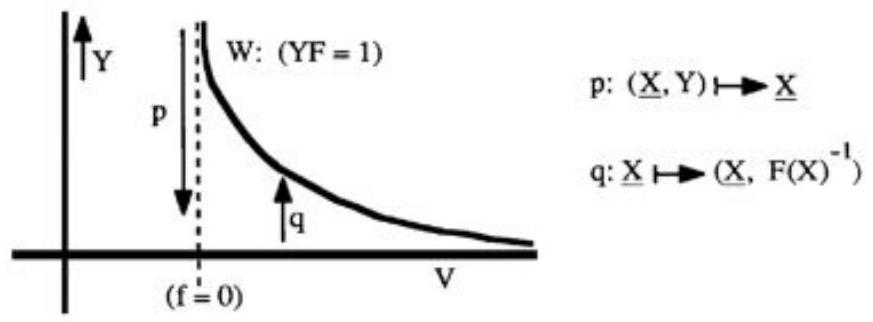
\includegraphics[max width=0.6\textwidth]{images/bo_d3lj80c601uc738kffi0_77_525_1233_873_322_0.jpg}
\end{center}
\hspace*{3em} 

图4.1: \(1/f\) 的图像

设 \(J = I(V) \subset  k[X_1, \ldots, X_n]\)，并选择 \(F \in  k[X_1, \ldots, X_n]\) 使得 \(f = F \pmod{I(V)}\).现在定义理想 \(I = (J, YF - 1) \subset  k[X_1, \ldots, X_n, Y]\)，并令
\[
W = V(I) \subset  {\mathbb{A}}^{n + 1}.
\]
容易验证，图中所示的投影映射 \(\pi: W \to V_f\) 和它的逆映射 \(\sigma: V_f \to W, P \mapsto (P, 1/f(P))\) 都是态射，从而建立了 \(W\) 与 \({V}_{f}\) 之间的同构.关于坐标环的结论包含在定理4.8(III)中.
\end{proof}

标准开集 \({V}_{f}\) 很重要，因为它们构成了 \(V\) 的Zariski拓扑的一个基：每个开集 \(U \subset  V\) 都是标准开集的并（因为每个闭集都形如 \(V(I) = \bigcap_{f \in I} V(f)\)）.因此，上述命题的意义在于，每个开集 \(U \subset  V\) 都是由仿射簇形式的开集 \({V}_{f}\) 拼接而成的.

\section{例子：三次曲线上的群律}

在第2章中，我们讨论了平面非奇异射影三次曲线 \(C \subset  {\mathbb{P}}^{2}\) 上的加法法则 \((A,B) \mapsto  A + B\).设 \({C}_{0} : (y^2 = x^3 + ax + b)\) 为一条非奇异仿射三次曲线.

\begin{center}
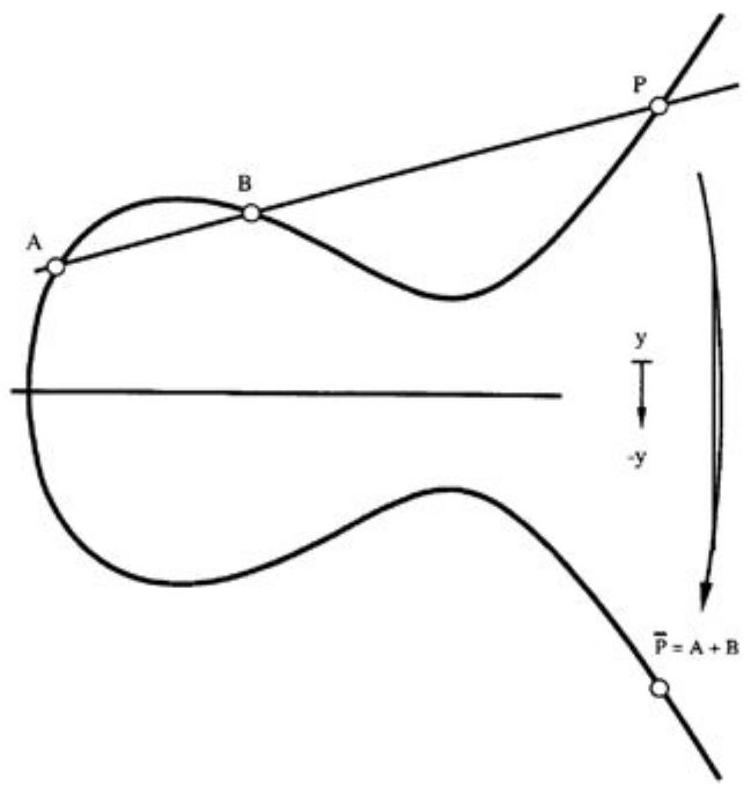
\includegraphics[max width=0.5\textwidth]{images/bo_d3lj80c601uc738kffi0_78_468_683_748_789_0.jpg}
\end{center}
\hspace*{3em} 

图4.2: 三次曲线上的群律作为态射

我们在此展示加法法则定义了一个有理映射 \(\varphi  : {C}_{0} \times  {C}_{0} \dashrightarrow {C}_{0}\)，且 \(\varphi\) 在其定义域内是一个态射.虽然我们不展开细节，但该论证可用于通过“连续性”给出群法则结合律的另一种证明，该证明适用于任意域.

不难看出（参见练习2.7），若 \(A = (x,y), B = (x',y')\) 且 \(x \neq  x'\)，则设 \(u = (y - y')/(x - x')\)，第三个交点为 \(P = (x'',y'')\)，其中
\[
x'' = f(x,y,x',y') = u^2 - (x + x'),
\]
\[
y'' = g(x,y,x',y') = u^3 + xu + y'.
\]
由于 \(x''\) 和 \(y''\) 是坐标 \((x,y), (x',y')\) 的有理函数，这表明 \(\varphi  : {C}_{0} \times {C}_{0} \dashrightarrow {C}_{0}\) 是一个有理映射.根据给定的公式，\(\varphi\) 在 \(x \neq  x'\) 处是一个态射，因为此时 \(u\) 的分母非零.

现在考虑 \(x = x'\) 的情况.如果 \(y = -y'\)，那么 \(x''\) 和 \(y''\) 应该是无穷大，这对应于直线 \(AB\) 在无穷远点 \(O\) 与射影曲线 \(C\) 相交.然而，如果 \(y = y' \neq  0\)（即 \(A=B\) 且不是2-挠点），则点 \(P = (x'',y'')\) 应该是良定义的.我们断言 \(f,g\) 在此类点上是正则的.为此，注意到
\[
y^2 = x^3 + ax + b \quad \text{且} \quad y'^2 = x'^3 + ax' + b,
\]
得到
\[
y^2 - y'^2 = x^3 - x'^3 + a(x - x').
\]
因此，作为 \({C}_{0} \times  {C}_{0}\) 上的有理函数，我们有等式
\[
u = \frac{y - y'}{x - x'} = \frac{x^2 + xx' + x'^2 + a}{y + y'}.
\]
观察第二个表达式的分母，可知只要 \(y \neq -y'\)，\(u\)（因此 \(f\) 和 \(g\)）就是正则的.

计算的结论是：加法律 \(\varphi  : {C}_{0} \times  {C}_{0} \dashrightarrow {C}_{0}\) 在点 \((A,B) \in  {C}_{0} \times  {C}_{0}\) 处是态射，当且仅当 \(A + B \neq  O\).

\section{第四章习题}

4.1 检验从本章开始到(4.8, I)的陈述对任意域 \(k\) 均成立.特别地，探究它们对有限域的含义.如果 \(k\) 不是代数闭的，请给出(4.8, II)的一个反例.

4.2 设 \(\varphi : {\mathbb{A}}^{1} \rightarrow  {\mathbb{A}}^{3}\) 是由 \(X \mapsto  (X, X^2, X^3)\) 给出的多项式映射.证明 \(\varphi\) 的像是代数子集 \(C \subset  {\mathbb{A}}^{3}\)，且 \(\varphi : {\mathbb{A}}^{1} \rightarrow  C\) 是一个同构.尝试推广此结论.

4.3 设 \({\varphi }_{n} : {\mathbb{A}}^{1} \rightarrow  {\mathbb{A}}^{2}\) 是由 \(X \mapsto  (X^2, X^n)\) 给出的多项式映射.证明：如果 \(n\) 是偶数，\({\varphi }_{n}\) 的像同构于 \({\mathbb{A}}^{1}\)，且 \({\varphi }_{n}\) 在原点之外是二对一的.如果 \(n\) 是奇数，证明 \({\varphi }_{n}\) 是双射，并给出一个有理逆映射.

4.4 证明两个仿射簇之间的态射 \(\varphi : X \rightarrow  Y\) 是 \(X\) 与其像 \(\varphi(X) \subset  Y\) 之间的同构，当且仅当诱导的同态 \(\Phi : k[Y] \rightarrow  k[X]\) 是满射.

4.5 设 \(C : \left( {{Y}^{2} = {X}^{3}}\right)  \subset  {\mathbb{A}}^{2}\) ；则

(a) 由 \(\left( {{T}^{2},{T}^{3}}\right)\) 给出的参数化 \(f : {\mathbb{A}}^{1} \rightarrow  C\) 是多项式映射；

(b) \(f\) 具有由 \(\left( {X,Y}\right)  \mapsto  Y/X\) 定义的有理逆映射 \(g : C \rightarrow  {\mathbb{A}}^{1}\) ；

(c) \(\operatorname{dom}g = C \setminus  \{ \left( {0,0}\right) \}\) ;

(d) \(f\) 和 \(g\) 给出逆同构 \({\mathbb{A}}^{1} \setminus  \{ 0\}  \cong  C \setminus  \{ \left( {0,0}\right) \}\) .

4.6 (i) 证明 \(g \circ  f\) 的定义域可能严格大于 \(\operatorname{dom}f \cap  {f}^{-1}\left( {\operatorname{dom}g}\right)\) .[提示:如果 \(g\) 和 \(f\) 是逆有理映射，这种情况可能发生；尝试Ex. 4.5中的 \(f\) 和 \(g\) .]

(ii) 多元微积分课程中常包含如函数 \(f\left( {x,y}\right)  = {xy}/\left( {{x}^{2} + {y}^{2}}\right)\) 的例子.解释为何当限制在通过(0,0)的任意光滑曲线时， \(f\) 是 \({C}^{\infty }\) ，但作为二维变量的函数却不连续.

4.7 设 \(C : \left( {{Y}^{2} = {X}^{3} + {X}^{2}}\right)  \subset  {\mathbb{A}}^{2}\) ；由 \(\left( {{T}^{2} - }\right.\)  \(1,{T}^{3} - T)\) 给出的熟悉参数化 \(\varphi  : {\mathbb{A}}^{1} \rightarrow  C\) 是多项式映射，但不是同构(为什么？).判断其限制 \({\varphi }^{\prime } : {\mathbb{A}}^{1} \setminus  \{ 1\}  \rightarrow  C\) 是否为同构:

\begin{center}
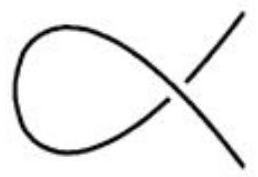
\includegraphics[max width=0.2\textwidth]{images/bo_d3lj80c601uc738kffi0_80_716_422_258_177_0.jpg}
\end{center}
\hspace*{3em} 

图4.3:带缺口的结点曲线

4.8 设 \(C : \left( {{Y}^{3} = {X}^{4} + {X}^{3}}\right)  \subset  {\mathbb{A}}^{2}\) ；证明 \(\left( {X,Y}\right)  \mapsto  X/Y\) 定义了有理映射 \(\psi  : C \rightarrow  {\mathbb{A}}^{1}\) ，其逆映射是多项式映射 \(\varphi  : {\mathbb{A}}^{1} \rightarrow  C\) ，参数化了 \(C\) .证明 \(\varphi\) 限制为同构

\[
{\mathbb{A}}^{1} \setminus  \{ 3\text{ pts. }\}  \cong  C \setminus  \{ \left( {0,0}\right) \} .
\]

4.9 设 \(V : \left( {{XT} = {YZ}}\right)  \subset  {\mathbb{A}}^{4}\) ；解释为何 \(k\left\lbrack  V\right\rbrack\) 不是唯一分解整环(UFD).(理解不难，但给出严格证明较难.) 若 \(f = X/Y \in  k\left( V\right)\) ，求 \(\operatorname{dom}f\) ，并证明其严格包含于闭子集 \(\left( {Y = 0}\right)  \subset  V\) .

4.10 设 \(f : {\mathbb{A}}^{1} \rightarrow  {\mathbb{A}}^{2}\) 由 \(X \mapsto  \left( {X,0}\right)\) 给出，且设 \(g : {\mathbb{A}}^{2} \rightarrow  {\mathbb{A}}^{1}\) 是由 \(\left( {X,Y}\right)  \mapsto  X/Y\) 给出的有理映射；证明复合映射 \(g \circ  f\) 在任何点都未定义.确定函数域 \(k\left( {\mathbb{A}}^{1}\right)\) 中 \({g}^{ * }\) 定义的最大子集.

4.11 定义并研究两个代数集的乘积的概念.更具体地，

(i) 若 \(V \subset  {\mathbb{A}}_{k}^{n}\) 和 \(W \subset  {\mathbb{A}}_{k}^{m}\) 是代数集，证明 \(V \times  W \subset  {\mathbb{A}}_{k}^{n + m}\) 也是代数集；

(ii) 举例说明 \(V \times  W\) 上的Zariski拓扑不是 \(V\) 和 \(W\) 上的积拓扑；

(iii) 证明若 \(V,W\) 不可约，则 \(\Rightarrow  V \times  W\) 也不可约；

(iv) 证明若 \(V \cong  {V}^{\prime }\) 和 \(W \cong  {W}^{\prime }\) ，则 \(V \times  W \cong  {V}^{\prime } \times  {W}^{\prime }\) .

4.12 (a) 证明任何在原点(0,0)处不正则的 \(f \in  k\left( {\mathbb{A}}^{2}\right)\) ，在经过(0,0)的曲线上的点处也不正则.

(b) 推断 \({\mathbb{A}}^{2} \setminus  \left( {0,0}\right)\) 不是仿射的.[提示:(a)中，利用 \(k\left( {\mathbb{A}}^{2}\right)  = k\left( {X,Y}\right)\) 是唯一分解整环(UFD) \(k\left\lbrack  {X,Y}\right\rbrack\) 的分式域，以及习题3.13(b)的结果；(b)中，假设 \({\mathbb{A}}^{2} \setminus  \left( {0,0}\right)\) 是仿射的，确定其坐标环；然后利用推论4.5得到矛盾.] 第三部分
